%! program = pdflatex

%\documentclass[12pt,a4paper]{memoir} % for a long document
\documentclass[12pt,a4paper]{memoir} % for a short document
\usepackage{graphicx}
\usepackage{enumitem}
    % See the ``Memoir customise'' template for some common customisations
    % Don't forget to read the Memoir manual: memman.pdf

\title{Final Report for ADT Scagram}
\author{}
    % \date{} % Delete this line to display the current date

    %%% BEGIN DOCUMENT
\begin{document}

\maketitle
\tableofcontents* % the asterisk means that the contents itself isn't put into the ToC

\chapter{Introduction}
This document explain the choices that where made in order to allow persistent storage of RDF data with some graph databases libraries.

This document first describe how the RDF are mapped to the graph database internal data.


\paragraph{Please note that the reference documentation is the javadoc of the source code: the purpose of this document is to provide the global structure of the framework and the motivations behind some implementation choices.}

\chapter{Mapping of RDF Data to Graph Database}
Since the graph databases do not support natively the storage of RDF data, a mapping must defined between the RDF data and the graph database ; \textit{ie} how the RDF data content and relationships are translated to and from the graph database storage used.
Since the performances on the requests is highly dependent on the implementation choices done in each graph database library\footnote{(\textit{eg} if the edges of the graph can be globally indexed or not, making a search of an edge linear or logarithmic in the size of the edges)}, the framework allows to specialize a mapping for each graph database.

\section{Architecture for the Mapping}

The architecture is made of a strategy pattern:
\begin{itemize}
\item[GdbDriver] defines a generic API allowing to (i) manipulate the graph database (open, close, etc.); (ii) add data from a Jena stream of data; (iii) read data from the database and return Corese objects.
\item A set of driver extending the GdbDriver abstract class, depending on the database used. Currently they are three implementations on OrientDb, TitanDb and Neo4j. Only the Neo4j driver is currently maintained.
\end{itemize}
The choice of the driver to use is made at runtime, depending on the value of the Java property \texttt{fr.inria.corese.tinkerpop.driver}. By default, the Neo4j driver is used.

\subsection{Graph Database Structure}
The graph used in the graph databases have the following two specificities that are used in the implementation:
\begin{itemize}
\item graph databases define a special property, called \textbf{label}, that is used to categorize vertices and edges.
\item properties, ie key/value pairs, can be set on edges and vertices.
\end{itemize}


\subsection{Abstract Class for the Mapping}
The abstract class defining the mapping is \texttt{fr.inria.corese.rdftograph.driver.GdbDriver}.
This class is divided in subsets of methods related to a given functionality the class is responsible for:

\begin{description}[align=left]
	\item [Graph Database Management] Include methods to open, close and commit;
	\item [RDF Storage] Functions to create RDF edges and vertices in the graph database. 
\end{description}

\subsubsection{Graph Database Management}
This functional group is made of three methods: 
\begin{description}[align=left]
	\item[openDatabase(dir)] This method opens a graph database in the directory \textit{dir}, previously created database by \textit{createDatabase};
	\item[createDatabase] This method first removes the content of the repository targeted for the database creation, then create the database and configure it if required. For example, the global indexex creation should be done in this method. 
	\item[closeDatabase] This method should close the database gracefully, \textit{ie} trying to commit before closing. 
	\item[commit] Self-explanatory method.
\end{description}

\subsubsection{RDF Storage}
These methods are responsible for the mapping of the RDF artefacts into graph database entities.
\begin{description}[align=left]
	\item[createRelationship] Allows for the creation in the graph database of the representation for a RDF triplet.
	\item[createOrGetNode(Value v)] allows to retrieve a RDF node given its value, or to create it if it was not already created. 
\end{description}

\section{Example of a Mapping Implementation: Neo4j}

    \subsection{General Representation}
In \textit{Neo4j}, the edges are only locally indexed, but not globally. 
That means it is quick to find an edge from a given node, but the search of an edge among all the edges is linear, becoming quickly intractable when the size of the graph is growing.


\subsection{Mapping of the RDF edges}
The R-edges are made of 4 elements, as depicted in figure~\ref{fig:anRdfEdge}:
\begin{itemize}
\item the \textit{predicate} ($p$ in the figure) stands for the relationship between two nodes;
\item the \textit{subject} ($s$ in the figure) of the predicate;
\item the \textit{object} ($o$ in the figure) of the predicate;
\item the \textit{graph} ($g$ in the figure) is optional and indicates that the predicate, subject and object are in a given namespace.
\end{itemize}

\begin{figure}[hbtp]
\centering
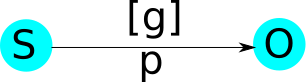
\includegraphics[scale=0.5]{figures/anRdfEdge.png}
\caption{an RDF edge}
\label{fig:anRdfEdge}
\end{figure}

 Due to the inefficiency of the global search for an edge in Neo4j, it has been chosen to map each RDF-edge as a Neo4j-node. In the following, N-node and N-edge stand for Neo4j node and edge respectively, while R-node and R-edge stands for RDF node and edge. 

\begin{figure}[hbtp]
\centering
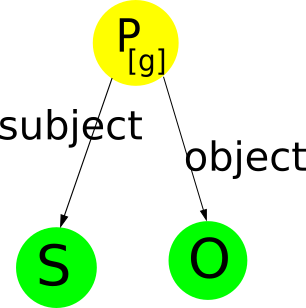
\includegraphics[scale=0.5]{figures/neo4jMapping.png}
\caption{Mapping in Neo4j of an RDF edge}
\label{fig:neo4jEdgeMapping}
\end{figure}

As depicted at figure~\ref{fig:neo4jEdgeMapping}:
\begin{itemize}
\item The R-nodes $s$ and $o$ are mapped to N-nodes of label \texttt{RDF_VERTEX_LABEL}. The mapping depends of the RDF type of the data and is described at~\ref{node_mapping}.
\item The R-edge $p$ (with an optional graph name $g$ ) is mapped to a N-node of label \textt{RDF_EDGE_LABEL}. 
\item The R-edges \texttt{subject} and \texttt{object} connect the node represeting $p$ to $s$ and $o$ respectively.
\end{itemize}

\subsubsection{Representation of the source and object nodes\label{node_mapping}}

\subsection{Graph Database Management Methods}
\begin{description}[align=left]
	\item[openDatabase] This method does nothing more than using the \textit{Neo4jGraph.open()}: ie, it only open an existing database;
	\item[closeDatabase] Closes a previously opened database.
	\item[createDatabase(String dbPath)] Deletes the content of the targeted directory, then initializes a database in dbPath.
	\item[commit] Force the commit of the pending data.
\end{description}

\subsection{RDF Data to Graph Data Management Methods}
\begin{description}[align=left]
\item[createRelationShip(s,o,p,properties)]
\item[getNode]
\item[createOrGetNode]
\end{description}

\subsection{Graph Data to Corese Methods}
\begin{description}[align=left]
\item[buildEdge] Low-level call defining how to build a Corese EdgeQuad from a data structure representing an RDF edge.
\item[buildNode] Low-level call defining how to build a Corese IDataType for an RDF node.

\end{description}

\end{document}
